
\section{Introduction}
The field at the bottom of the Eigenmath window is for entering
calculations that get evaluated right away.

\begin{center}
\begin{tikzpicture}
\node at (0,0) {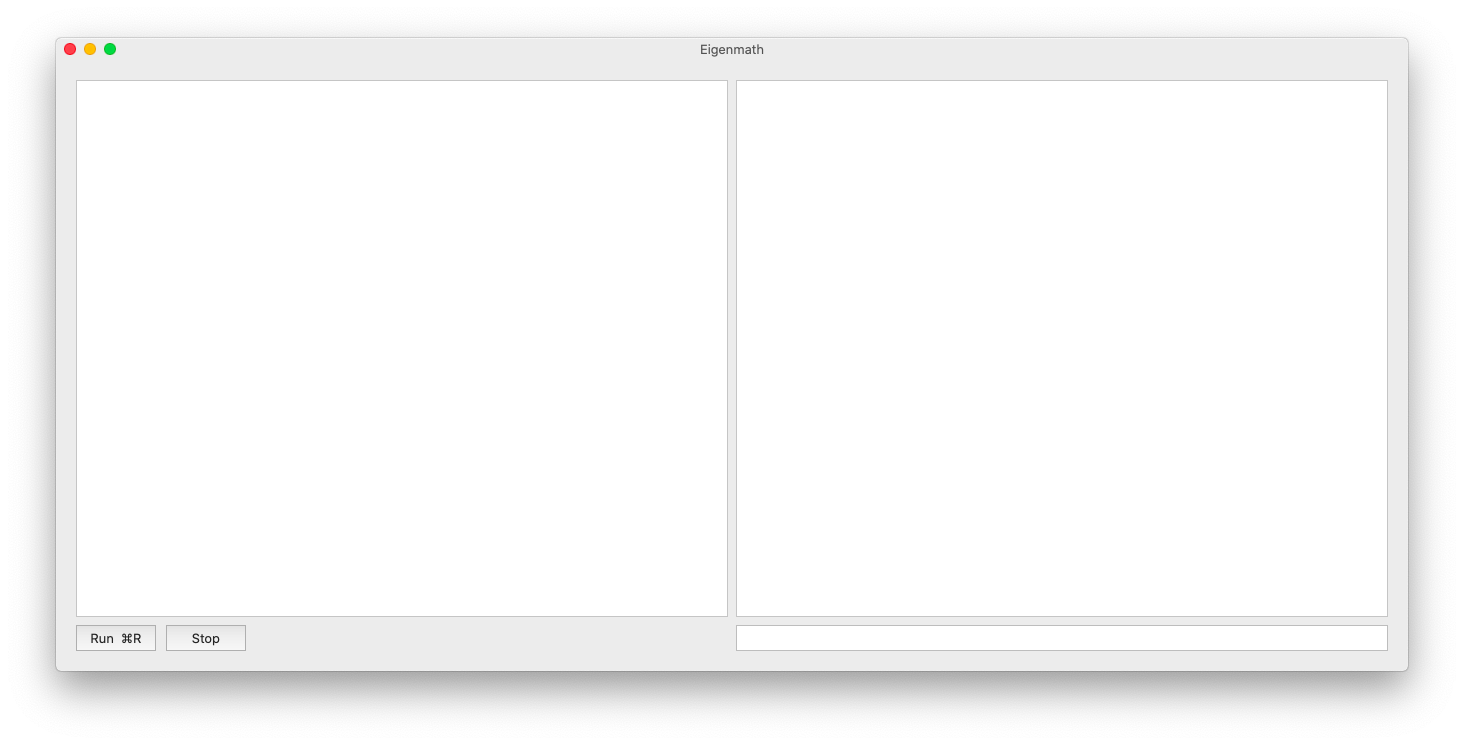
\includegraphics[scale=0.2]{face.png}};
\draw[red,thick] (2.3,-1.85) ellipse (2.5cm and 0.5cm);
\end{tikzpicture}
\end{center}

For example, let us check the following
arithmetic from Vladimir Nabokov's autobiography {\it Speak, Memory.}

\begin{quote}
A foolish tutor had explained logarithms to me much too early, and I had
read (in a British publication, the {\it Boy's Own Paper}, I believe)
about a certain Hindu calculator who in exactly two seconds could find the
seventeenth root of, say,
%$3529471145760275132\\301897342055866171392$
% Use math mode so htlatex does not break the number
3529471145760275132301897342\\055866171392
(I am not sure I have got this right; anyway the root was 212).
\end{quote}

We can check Nabokov's arithmetic by entering the following calculation.

\begin{Verbatim}[formatcom=\color{blue}]
212^17
\end{Verbatim}

After pressing the return key, Eigenmath displays the following result.

$3529471145760275132301897342055866171392$

So Nabokov did get it right after all.
Now let us see if Eigenmath can find the
seventeenth root of this number, like the Hindu calculator could.

\begin{Verbatim}[formatcom=\color{blue}]
N = 212^17
N^(1/17)
\end{Verbatim}

Eigenmath displays the following result.

$212$

When a symbol is assigned a value, such as $N$ above,
no result is printed.
To see the value of a symbol, just evaluate it.

\begin{Verbatim}[formatcom=\color{blue}]
N
\end{Verbatim}

$N=3529471145760275132301897342055866171392$

The previous example shows a convention that will be used throughout
this manual.
That is, the color blue indicates something that the user should type.
The computer response is shown in black.
